%%%%%%%%%%%%%%%%%%%%%%%%%%%%%%%%%%%%%%%%%%%%%%%%%%%%%%%%%%%%%%%%%%%%%%%%%%
%%LaTeX template for papers && theses									%%
%%Done by the incredible ||Z01db3rg||									%%
%%Under the do what ever you want license								%%
%%%%%%%%%%%%%%%%%%%%%%%%%%%%%%%%%%%%%%%%%%%%%%%%%%%%%%%%%%%%%%%%%%%%%%%%%% 

%start preamble
\documentclass[paper=a4,fontsize=11pt]{scrartcl}%kind of doc, font size, paper size
\usepackage[ngerman]{babel}%for special german letters etc			
%\usepackage{t1enc} obsolete, but some day we go back in time and could use this again
\usepackage[T1]{fontenc}%same as t1enc but better						
\usepackage[utf8]{inputenc}%utf-8 encoding, other systems could use others encoding
%\usepackage[latin9]{inputenc}			
\usepackage{amsmath}%get math done
\usepackage{amsthm}%get theorems and proofs done
\usepackage{graphicx}%get pictures & graphics done
\graphicspath{{pictures/}}%folder to stash all kind of pictures etc
\usepackage{amssymb}%symbolics for math
\usepackage{amsfonts}%extra fonts
\usepackage []{natbib}%citation style
\usepackage{caption}%captions under everything
\usepackage{listings}
\usepackage[titletoc]{appendix}
\numberwithin{equation}{section} 
\usepackage[printonlyused,withpage]{acronym}%how to handle acronyms
\usepackage{float}%for garphics and how to let them floating around in the doc
\usepackage{cclicenses}%license!
\usepackage{xcolor}%nicer colors, here used for links
\usepackage{wrapfig}%making graphics floated by text and not done by minipage
\usepackage{dsfont}
\usepackage{stmaryrd}
\usepackage{geometry}
\usepackage{hyperref}
\usepackage{fancyhdr}
\usepackage{menukeys}
\usepackage{multicol}

%settings colors for links
\hypersetup{
    colorlinks,
    linkcolor={blue!50!black},
    citecolor={blue},
    urlcolor={blue!80!black}
}

\definecolor{pblue}{rgb}{0.13,0.13,1}
\definecolor{pgreen}{rgb}{0,0.5,0}
\definecolor{pred}{rgb}{0.9,0,0}
\definecolor{pgrey}{rgb}{0.46,0.45,0.48}

\pagestyle{fancy}
\lhead{Netzwerke Übung (SoSe 2019)}
\rhead{FB 4 -- Angewandte Informatik\\ HTW-Berlin}
\lfoot{Übungsblatt 3 -- Routing}
\cfoot{}
\fancyfoot[R]{\thepage}
\renewcommand{\headrulewidth}{0.4pt}
\renewcommand{\footrulewidth}{0.4pt}


\lstdefinestyle{Bash}{
  language=bash,
  showstringspaces=false,
  basicstyle=\small\sffamily,
  numbers=left,
  numberstyle=\tiny,
  numbersep=5pt,
  frame=trlb,
  columns=fullflexible,
  backgroundcolor=\color{gray!20},
  linewidth=0.9\linewidth,
  %xleftmargin=0.5\linewidth
  upquote=true,
  columns=fullflexible,
  literate={*}{{\char42}}1
         {-}{{\char45}}1
}

\newlength\labelwd
\settowidth\labelwd{\bfseries viii.)}
\usepackage{tasks}
\settasks{counter-format =tsk[a].), label-format=\bfseries, label-offset=3em, label-align=right, label-width
=\labelwd, before-skip =\smallskipamount, after-item-skip=0pt}
\usepackage[inline]{enumitem}
\setlist[enumerate]{% (
labelindent = 0pt, leftmargin=*, itemsep=12pt, label={\textbf{\arabic*.)}}}

\pdfpkresolution=2400%higher resolution

%%here begins the actual document%%
\newcommand{\horrule}[1]{\rule{\linewidth}{#1}} % Create horizontal rule command with 1 argument of height

\DeclareMathOperator{\id}{id}

\begin{document}
\begin{center}
\Large{\textbf{Übungsblatt 03 -- Routing}}
\end{center}
\textbf{Hilfreiche Programme:}
\begin{multicols}{3}
\begin{itemize}
	\item ifconfig, ip addr
	\item ip link
	\item route/ip route
	\item sysctl
	\item netstat 
	\item ping
\end{itemize}
\end{multicols}
	
\begin{center}\Large{\textbf{Aufgabe A -- Umsetzung des Routings}}\end{center}\vskip0.25in
%\setlist[enumerate, 1]{itemsep=\baselineskip}
Setzen Sie das aus der Planung hervorgegangene Netzwerk (bzw. die Netzwerke) um.
\begin{enumerate}
	\item Vergleichen Sie innerhalb Ihrer Gruppe die Ergebnisse der Hausaufgaben, sodass Sie Ihr Vorgehen koordinieren können.
	\item \textbf{Für die Hosts:}\\
	\begin{tasks}(1)
		\task Beschriften Sie die aus den Hausaufgaben hervorgegangene Skizze mit den in der Gruppe zu vergebenen IP-Adressen.
		\task Setzen Sie die IP-Adressen und Routen mithilfe der Kommandos \emph{ip add} und \emph{ip route [add|delete|replace]} aus dem \emph{iproute2}-Werkzeugkasten bzw. den Networking-Tools \emph{ifconfig} und \emph{route add}.\\
		Achten Sie darauf, ob Sie ein Default-Gateway definieren oder ein \glqq herkömmliches\grqq\ Gateway! Beides ist möglich, jedoch erweitern Sie bald Ihr Netzwerk, wodurch sich dies ändern könnte.
		\task Analysieren Sie die Ihnen vorliegende Routing-Tabelle. Was bedeuten die Einträge? Bzw. entspricht die Ausgabe Ihren Erwartungen?
	\end{tasks}
	\item \textbf{Für den Router:}\\
	Der Router benötigt eine etwas andere Konfiguration. 
	\begin{tasks}(1)
		\task Konfigurieren Sie am Router die IP-Adressen des Netzwerkadapters. Wenn Ihr Router zwischen zwei Netzwerken vermittelt, sollte dieser beide Netzwerke kennen. D.h. Ihr Router ist Teilnehmer an beiden Netzwerken und benötigt zwei IP-Adressen, für jedes Netzwerk eine.\\
		Anm.: Gewöhnlich hat der Router die erste verfügbare Adresse im Netzwerk, beachten Sie dennoch die Netz- und Broadcast-Adresse.
		\task Versuchen Sie den Router aus beiden Netzwerken via \emph{ping} zu erreichen.
		\task Testen Sie welche der anderen IP-Adressen Sie nun anpingen können und welche nicht.
	\end{tasks}
	\item Sie können mithilfe eines kleine Chats testen, ob Pakete tatsächlich auf dem Router ankommen. Dafür basteln Sie eine kleine  Client-Server-Lösung. Beide Seiten nutzen das Tool \emph{netcat -- \emph{nc}}. Das Listing \ref{netcat_server} zeigt die Seite des Servers. Dieser Stellt den Server bereit, der Client darf sich anschließend mithilfe eines \emph{Sockets (Tupel aus IP-Adresse und Port)} verbinden (s. Listing \ref{netcat_client}). 
		
	\begin{lstlisting}[style=Bash, language=Bash, label={netcat_server}]
#Server port > 1024 
nc -l -p <port_number> <ip_of_server>
#example
nc -l -p 4711 10.0.0.1
		\end{lstlisting}
		
		\begin{lstlisting}[style=Bash, language=Bash, label={netcat_client}]
#Client 
nc <ip_of_server> <port_number>
#example
nc 10.0.0.1 4711
		\end{lstlisting}
		\item \textbf{Alternativ:} Wenn Sie bereits mit Wireshark gearbeitet haben, können Sie auch dies benutzen um festzustellen, ob die Pakete korrekt ankommen. 
	\item \textbf{Router: Forwarding}\\
	Im Idealfall sollten Sie den Router auf beiden IP-Adressen erreichen können -- andere Rechner außerhalb ihres Netzes antworten Ihnen nicht (Sie können dies ruhig austesten!).\\
	Das Weiterleiten von Paketen muss auf dem Router explizit erlaubt werden, dies hat Sicherheitsgründe -- ansonsten könnten Pakete von Fremden im Netz beliebig versendet werden (Bspw.: Wenn Sie in Ihrem Notebook neben ihrem WiFi noch eine WWAN-Karte für teure LTE-Verbindugen betreiben, könnten andere Teilnehmer \glqq kostengünstig\grqq\ mitsurfen.)
	\begin{tasks}(1)
		\task Schauen Sie sich die Routing-Tabelle auf dem Router an. Welche Informationen können Sie diesem entnehmen?
        	\task Muss am Router eine Anpassung der Routing-Tabelle vorgenommen werden?
        	\task Aktivieren Sie das Forwarding im Betriebssystem des Routers. Ihre Umsetzung \textbf{soll keine persistente Lösung} sein! 
		\task Testen Sie jeweils mit einem \emph{ping} aller beteiligten Rechner, welche Netzwerke und IP-Adressen Sie erreichen können und welche nicht.
		\task \textbf{Wenn etwas nicht funktioniert:} Notieren Sie sich auftretende Fehlermeldungen und vergleichen Sie deren Ursache mit Ihren Recherchen aus den Hausaufgaben.
		\task Nutzen Sie erneut den Chat-Server mit \emph{netcat} um zu überprüfen, ob Ihr Netzwerk korrekt funktioniert.
	\end{tasks}
\end{enumerate}

\begin{center}\Large{\textbf{Aufgabe B -- Umsetzung des Backbones}}\end{center}\vskip0.25in
Sie erweitern nun das vorhandene Netzwerk dergestalt, dass ein weiterer Rechner aus jeder Reihe zum Router umgebaut wird. Wenn genug Raspberry Pis vorhanden sind, kann auch ein zusätzlicher Raspberry Pi an den Switch angeschlossen werden. Der neue Router soll alle Pakete, die an Rechner außerhalb des eigenen Netzes (Bankreihe) gehen, in die anderen Reihen weiterleiten können. Somit können Sie dann jeden beliebigen Raspberry Pi im Labor anpingen. Die Router sorgen dafür, dass alle Pakete über das \glqq Backbone\grqq\ zu ihrem Ziel geleitet werden. Im wesentlichen soll das Netzwerk Abbildung \ref{backbone} entsprechen. 
\begin{figure}[H]
	\center
	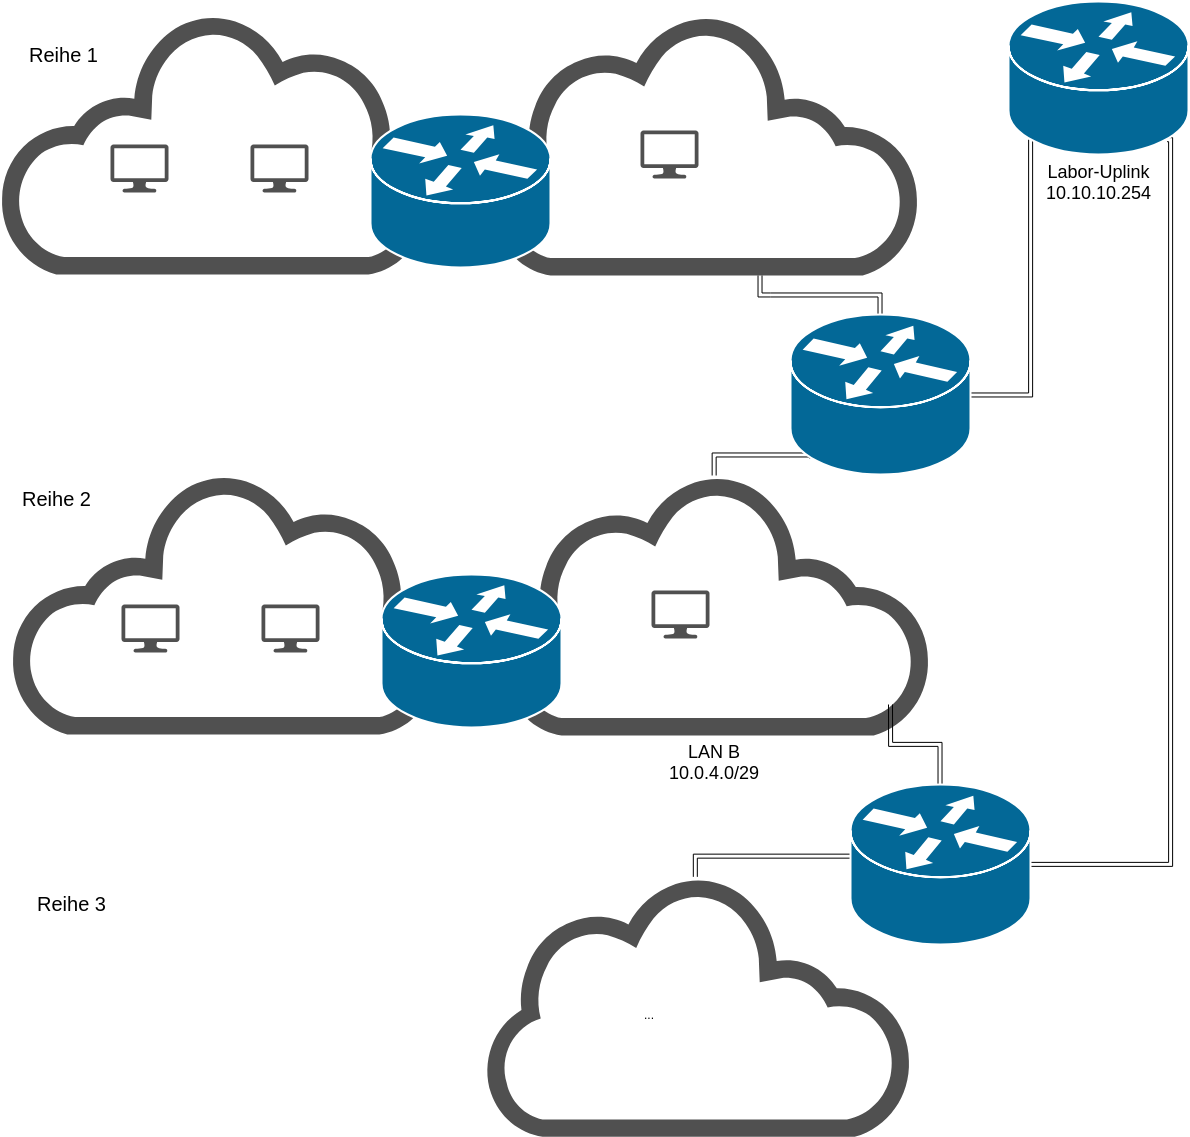
\includegraphics[scale=0.2]{backbone}
	\caption{Backbone-Netzwerk}
	\label{backbone}
\end{figure}
\begin{table}[H]
\caption{Adressschema für das Labor}
\label{adress_scheme}
\centering
\begin{tabular}{|c|c|}\hline
 & \textbf{IP  || IP-Range} \\ \hline
 $LAN_X$ & 10.0.$X$.Y/Size \\ \hline
 Backbone & 10.10.10.100 + $\rho$ \\ \hline
 Labornetz & 10.0.0.0/8 \\ \hline
 Uplink & 10.10.10.254 \\ \hline
 DNS & 10.10.10.254 \\ \hline
\end{tabular}
\end{table} 
\vskip0.05in ~\\
\textbf{Achtung:} Da es in dem Backbone-Netz fünf gleichwertige Router gibt, können Sie hier nicht mit \glqq Default-Routen\grqq\ arbeiten! Sie müssen auf den Backbone-Rechnern nun mehrere explizite Routen mit einem Zielnetzwerk und zugehöriger Subnetzmaske eintragen.
\begin{enumerate}
	\item Aufsetzen des Backbones:
	\begin{tasks}(1)
		\task Wählen Sie einen Rechner aus Ihrer Reihe der noch nicht als Router fungiert. Geben Sie diesem Router eine zweite IP-Adresse 10.10.10.X, wobei $X=100 + \rho$ ist und $\rho$ Ihrer Reihe entspricht.\\
		\task Aktivieren Sie auf dem Backbone ebenfalls das Forwarding.
		\task Tragen Sie alle Routen zu den anderen Reihen ein. Tragen Sie ebenfalls eine Route in das Subnetz für das $LAN_x$ ein, in dem der Backbone-Router selbst nicht Teilnehmer ist.
		\task Prüfen Sie mit \emph{ping}, ob Sie verschiedene Rechner innerhalb, sowie außerhalb Ihres Netzwerkes erreichen können -- bei welchen Rechner(n) klappt es und bei welchen nicht?
		\task Überprüfen Sie die Routen Ihrer Hosts! Haben die einfachen Hosts entsprechende Default-Routen? Hat Ihr Router eine Default-Route? Setzen Sie die Routen entsprechend, sodass im Anschluss alle Hosts sich untereinander erreichen können, als auch den Router und den Backbone-Router.
		\task Was müssen Sie jetzt noch an der Konfiguration einer oder aller anderen Rechner Ihrer Reihe anpassen, damit sich wirklich alle Rechner anpingen können.
		\task Befragen Sie als Hilfestellung den aktuellen Routing-Tabelle Ihres Betriebssystems. Sie können hierfür die Tools \emph{ip route, route, netstat -r} nutzen.
		\task Prüfen Sie mit \emph{ping} ob Sie jetzt wirklich alle Rechner erreichen können.
		\task Prüfen Sie mit \emph{Wireshark} auf dem neuen Backbone-Router, ob auch alle Pakete wirklich über diesen Rechner geleitet werden. Sie sollen ausschließen könne, dass irgendein Rechner eine \glqq Abkürzung\grqq\ nimmt.
		\task Sie können erneut den Chatserver mit \emph{netcat} betreiben, um sich zu vergewissern, dass Ihr Netzwerk funktioniert.
	\end{tasks}
\end{enumerate}

\begin{center}\Large{\textbf{Aufgabe C -- Einrichtung des Uplinks}}\end{center}\vskip0.25in
Seitdem Sie den DHCP-Dienst auf den Raspberry Pis ausgeschalteten, haben Sie keinen Uplink ins Internet mehr. Das soll sich mit dieser Aufgabe ändern.
\begin{enumerate}
	\item Richten Sie die Verbindung zum Uplink ein, sodass alle Raspberry Pis Ihres Netzwerkes eine Verbindung ins Internet bekommen.
	\begin{tasks}
		\task Erweitern Sie den Backbone-Router, sodass dieser den Uplink im Labor nutzen kann. Der Uplink ist auf dem Server im Dell-Rack untergebracht und besitzt die IP-Adresse: \url{10.10.10.254}. Wie Sie bereits vermuten werden, muss Ihr Router nun die Pakete in dieses Netz bzw. an diesen Knoten weiterleiten können. Konfigurieren Sie entsprechend Ihren Router zunächst mit den Ihnen bekannten Tools.
		\task Welche Art Route müssen Sie auf dieses Gateway konfigurieren? \textbf{Hinweis:} Alle Pakete, die nicht an die Netzwerke des Labors adressiert sind, sollten dieses Gateway passieren.
  		\task Befragen Sie als Hilfestellung den aktuellen Routing-Tabelle Ihres Betriebssystems. Sie könne hierfür die Tools \emph{ip route, route, netstat -r} nutzen.
  		\task Setzen Sie auf Ihrem Backbone das Network-Address-Translation mithilfe von \emph{iptables} um.
 		\task Da auf dem Uplink bereits ein DNS-Server arbeitet, müssen Sie sich keine Sorgen hierüber machen. Sie sollten nun sowohl IP-Adressen als auch Host-Names adressieren können.\\
 		Anmerkung: Die Auflösung von Hostnames kann evtl. etwas dauern, da das Betriebssystem erst die änderung in der Datei \path{/etc/resolv.conf} anpassen muss.
 		\task Versuchen Sie die Website des Instituts für Mathematik und Informatik der Freien Universität Berlin anzupingen.
 		(\url{mi.fu-berlin.de})
\end{tasks}
\end{enumerate}

\begin{center}\Large{\textbf{Aufgabe D -- IPv6}}\end{center}\vskip0.25in
Da \emph{IPv4} ein etwas betagteres Protokoll ist und Sie Fit für die Zukunft sein sollten, sollen Sie abschließend Ihr Netzwerk mittels \emph{IPv6} umsetzen. Da \emph{IPv6} eine wesentlich größere IP-Range besitzt ist in der Nachfolgenden Tabelle ein mögliches Adressschema aufgezeigt. Auch hier gilt: \emph{IPv6} hat mehr Adressen, was Sie jedoch nicht dazu verleiten soll, verschwenderisch damit umzugehen!
\begin{table}[H]
\centering
\begin{tabular}{ll}
 Prefix/L & fd  \\
 Global ID & 0da5a0170a \\
 Subnet ID &  5fd7\\
 Combined/CID & fd0d:a5a0:170a:5fd7::/64 \\
 IPv6 addresses & fd0d:a5a0:170a:5fd7:xxxx:xxxx:xxxx:xxxx 
\end{tabular}
\end{table}
Sie sollen im Folgenden ein statisches \emph{IPv6}-Netzwerk umsetzen. Ein Routing außerhalb unseres Labornetzwerkes ist leider nicht möglich, da die HTW-Berlin momentan kein \emph{IPv6} einsetzt.
\begin{enumerate}
	\item Adaptieren Sie Ihren Netzwerkaufbau von \emph{IPv4} auf \emph{IPv6}. D.h. der grundsätzliche Aufbau des Netzwerkes soll nicht verändert werden, Ihr Netzwerk soll um die Möglichkeit von \emph{IPv6} erweitert werden.
	\item Gehen Sie sicher, dass keine Adressdoppelung vorkommen. Es ist ausreichend, wenn jede Bankreihe eine eindeutige Netzadresse besitzt, Sie müssen nicht innerhalb einer Bankreihe zwei Subnetze aufspannen.
	\item Vergeben Sie in Ihrem Netzwerk entsprechende Adressen. Vergessen Sie nicht entsprechende Adressen für die Router zu setzen.
	\item Setzen Sie Routen, sodass die Raspberry Pis sich über ihre LANs hinweg erreichen.
	\item Testen Sie Ihre Netzwerke mit \emph{ping}.
\end{enumerate}

\begin{center}\Large{\textbf{Reset}}\end{center}\vskip0.25in
\begin{enumerate}
\item \textbf{Sofern Sie keine eigene SD-Karte nutzen:} Setzen Sie die Einstellungen des Raspberry Pis bzw. des Betriebssystems zurück die Sie vorgenommen haben! D.h. setzen Sie das Betriebssystem auf den initialen Zustand samt \emph{dhcp} zurück. Haken Sie zumindest folgende Liste ab:
\begin{itemize}
	\item Eigene IP-Config zurücksetzen:
	\begin{itemize}
		\item \path{/etc/network/interfaces}
		\item Bash-Script: \emph{reset\_network\_config.sh}
	\end{itemize}
	\item Routing/Forwarding:
	\begin{itemize}
		\item Keine persistenten Routen vorhanden?
		\item Forwarding deaktiviert? 
		\item \path{/etc/systctl.conf}
		\item \path{/proc/sys/net/ipv4/ip_forward}
	\end{itemize}
	\item DNS
	\begin{itemize}
		\item DNS Einträge verändert?
		\item \path{/etc/resolv.conf}
		\item \emph{reset\_hosts.sh}
	\end{itemize}
	\item DHCPcd:
	\begin{itemize}
		\item \emph{sudo systemctl enable dhcpcd}
		\item bzw. \emph{nw\_default.sh}
	\end{itemize}
\end{itemize}
\end{enumerate}
\end{document}